\section*{Supplementary Note 9: Prompts}\label{appendix:prompts}
We showcase all of the LLM prompts used in RDMA below.

\begin{figure}[h!]
    \centering
    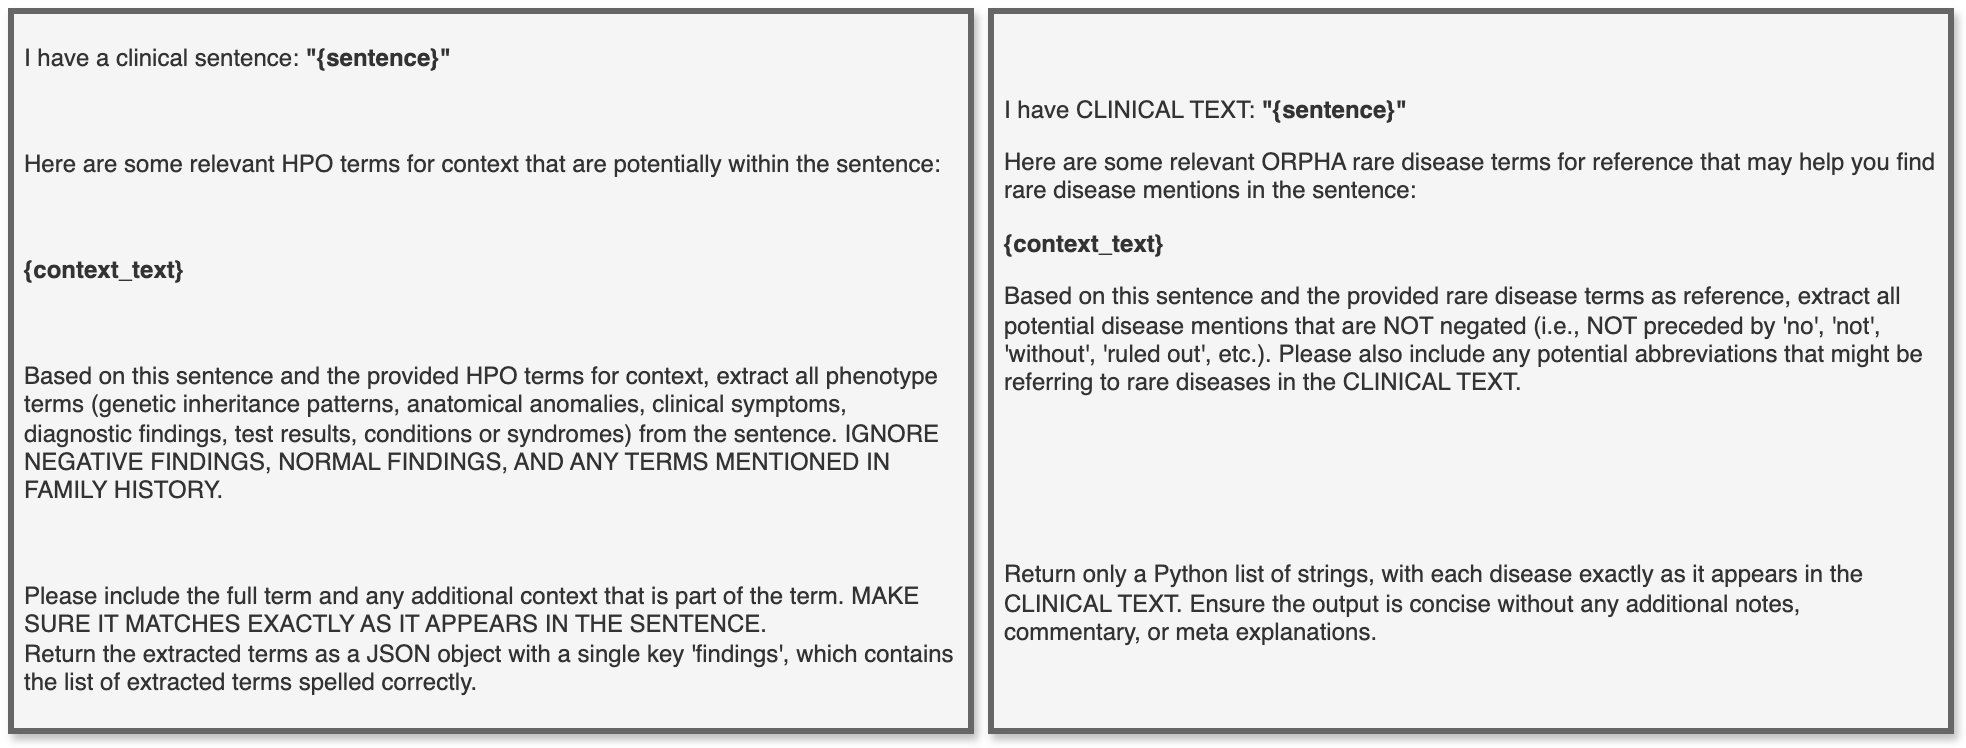
\includegraphics[width=1.0\textwidth]{figs/prompts/RetrievalExtractionPrompt.drawio.png}
    \caption{\textbf{Entity Extraction Prompts.} We showcase both HPO extraction (left) and Rare Disease extraction (right) prompts here.}
    \label{fig:EntityExtractionPrompt}
\end{figure}

\subsection{HPO Verification and Matching Prompts} \label{appendix: HPO prompts}
We showcase all of the prompts used for HPO extraction here. 

\begin{figure}[h!]
    \centering
    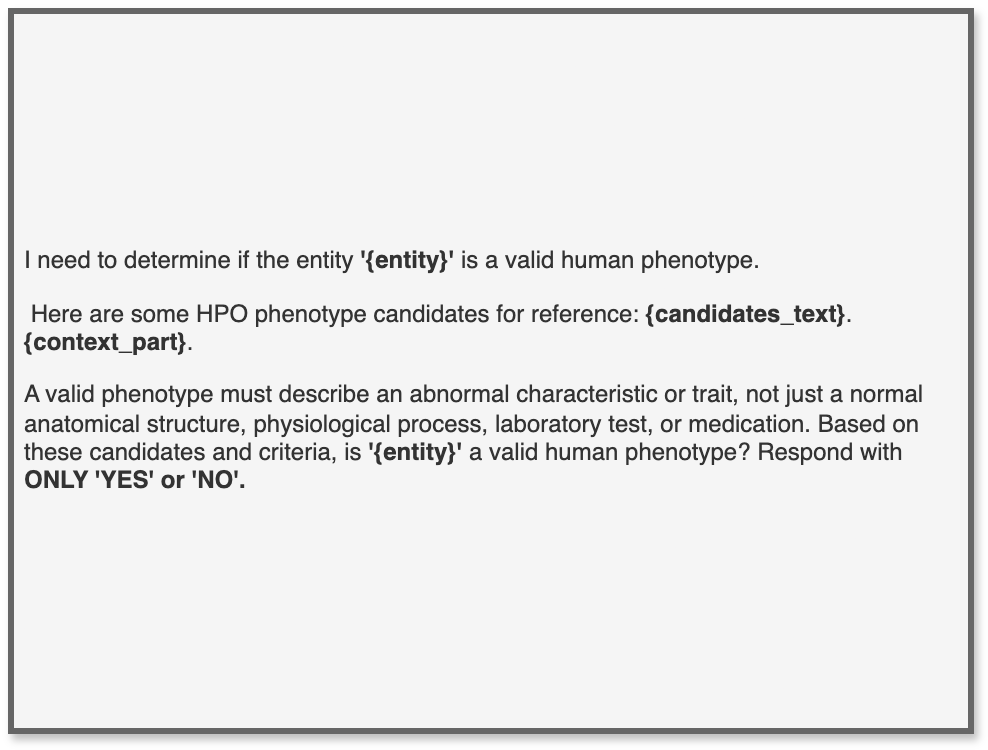
\includegraphics[width=0.8\textwidth]{figs/prompts/hpo/DirectPhenotype.drawio.png}
    \caption{\textbf{Verifying an Entity is a Phenotype.} This reasoning step is used repeatedly in verifying all phenotype implications, whether done by a lab test or a generated implication. }
    \label{fig:DirectPhenotype}
\end{figure}

\begin{figure}[h!]
    \centering
    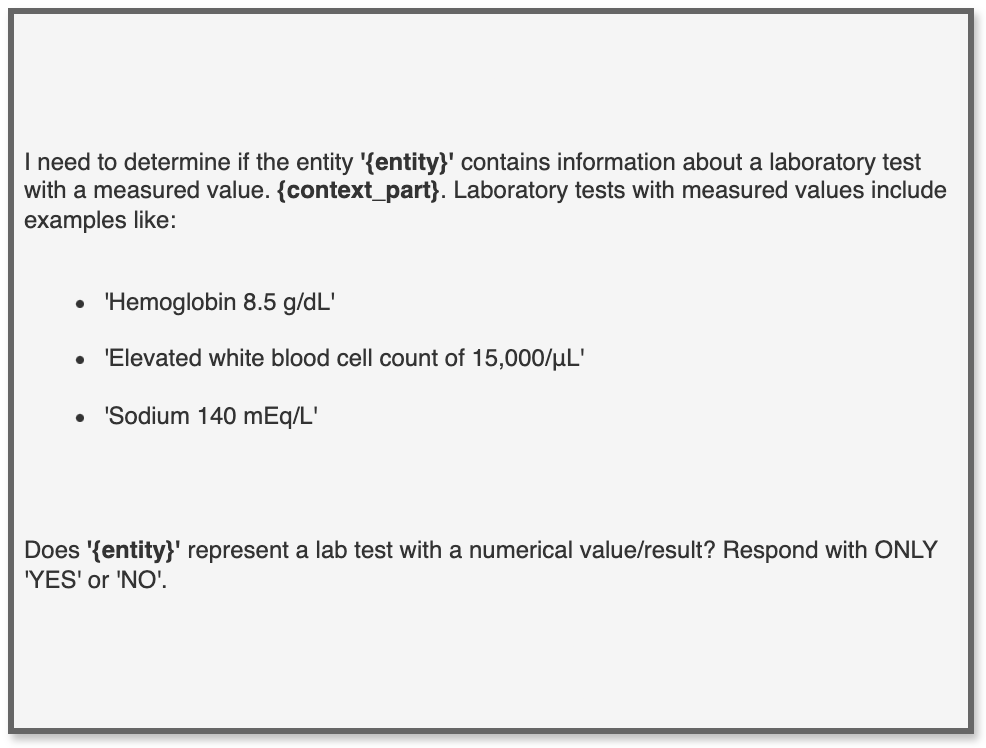
\includegraphics[width=0.8\textwidth]{figs/prompts/hpo/LabTestsCheckPrompt.drawio.png}
    \caption{\textbf{Lab Test Check.} LLMs are asked to see if an entity is indicative of a lab test. }
    \label{fig:LabTestsCheck}
\end{figure}

\begin{figure}[h!]
    \centering
    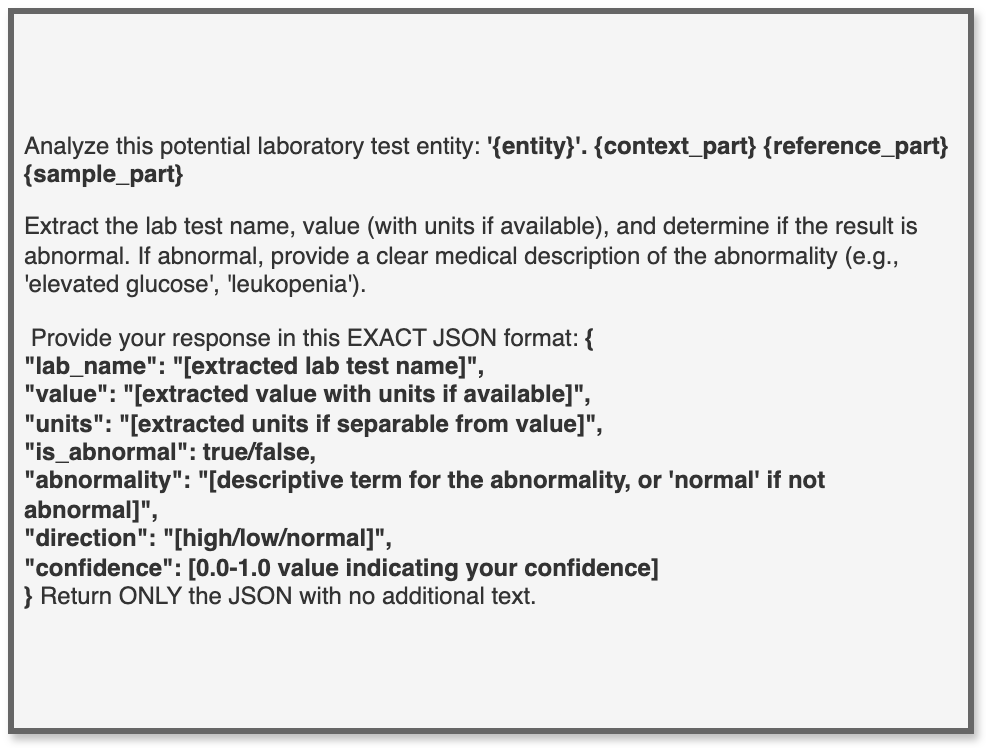
\includegraphics[width=0.8\textwidth]{figs/prompts/hpo/LabTestsAnalysis.drawio.png}
    \caption{\textbf{Lab Test Implication.} LLMs are asked to determine if a lab event indicates an abnormality in the patient.}
    \label{fig:LabTestsAnalysis}
\end{figure}


\begin{figure}[h!]
    \centering
    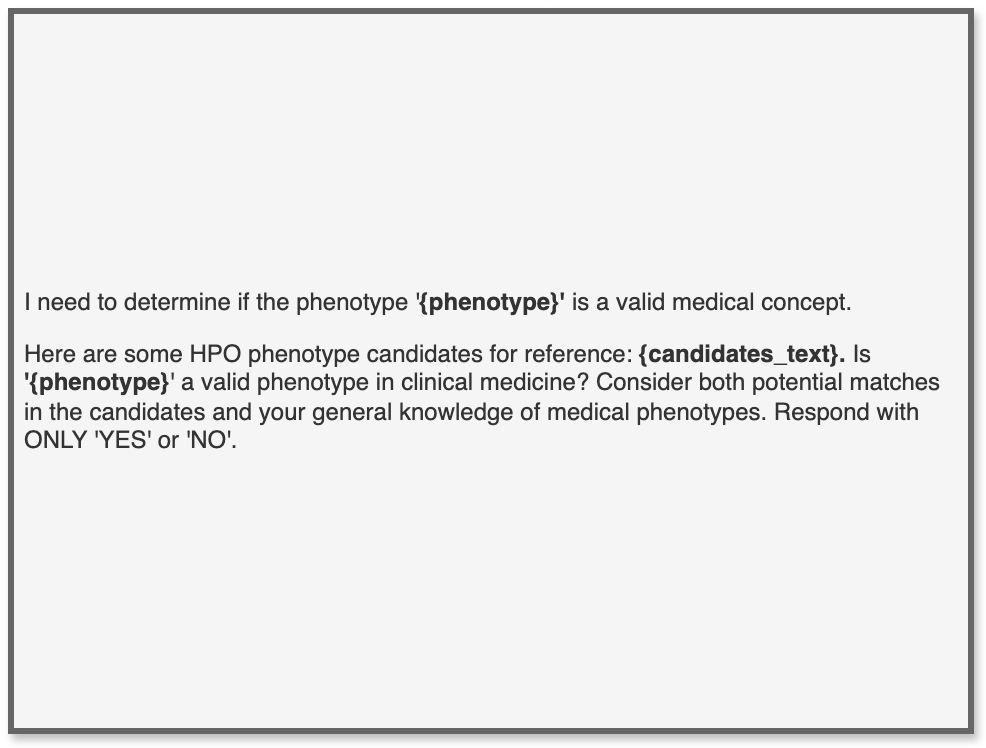
\includegraphics[width=0.8\textwidth]{figs/prompts/hpo/PhenotypeCorrectnessCheck.drawio.png}
    \caption{\textbf{Variant of Phenotype Verification.} This prompt is used to double check if an implied lab test phenotype is within the HPO ontology.}
    \label{fig:PhenotypeCorrectnessCheck}
\end{figure}


\begin{figure}[h!]
    \centering
    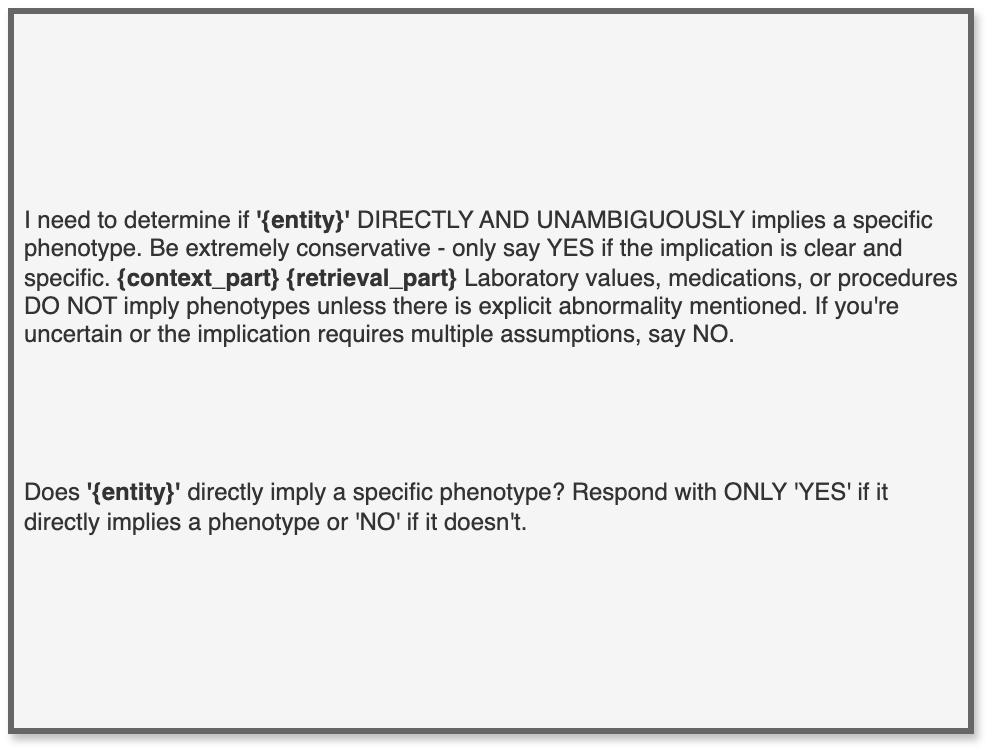
\includegraphics[width=0.8\textwidth]{figs/prompts/hpo/PhenotypeImplicationCheck.drawio.png}
    \caption{\textbf{Entity Implies Phenotype Check.} LLM is asked to check if an entity implies the possibility of a phenotype.}
    \label{fig:CheckIfImpliesPhenotypet}
\end{figure}

\begin{figure}[h!]
    \centering
    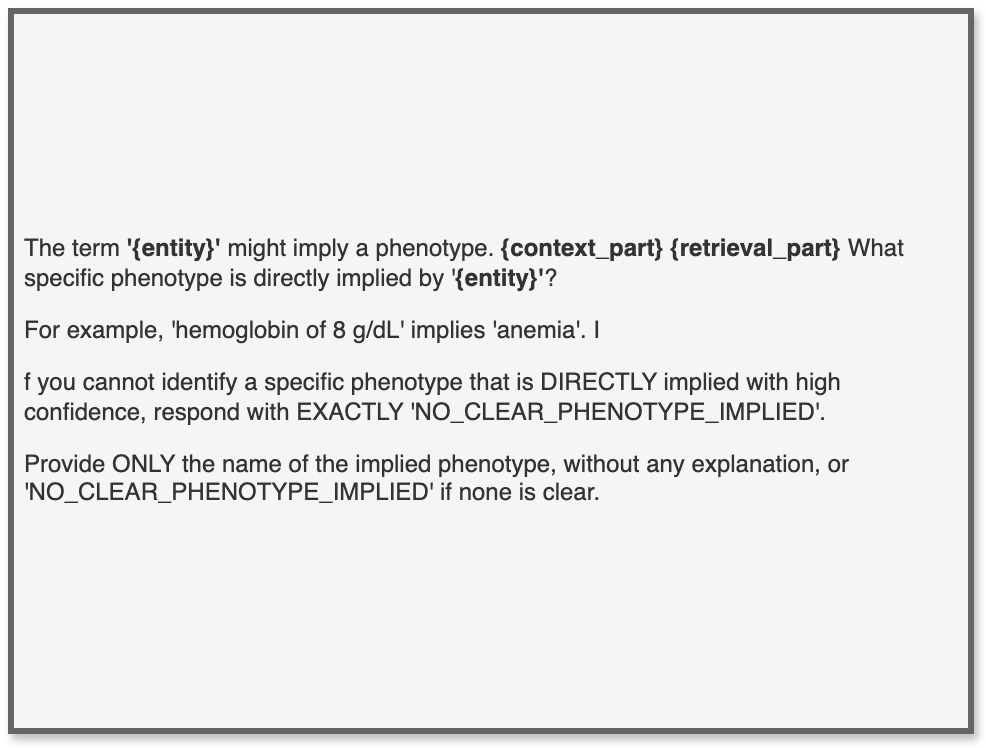
\includegraphics[width=0.8\textwidth]{figs/prompts/hpo/PhenotypeImplicationGeneration.drawio.png}
    \caption{\textbf{Phenotype Implication Generation.} The LLM is asked to generate or predict what the implied phenotype is based on context and the entity.}
    \label{fig:PhenoImplicationGeneration}
\end{figure}

\begin{figure}[h!]
    \centering
    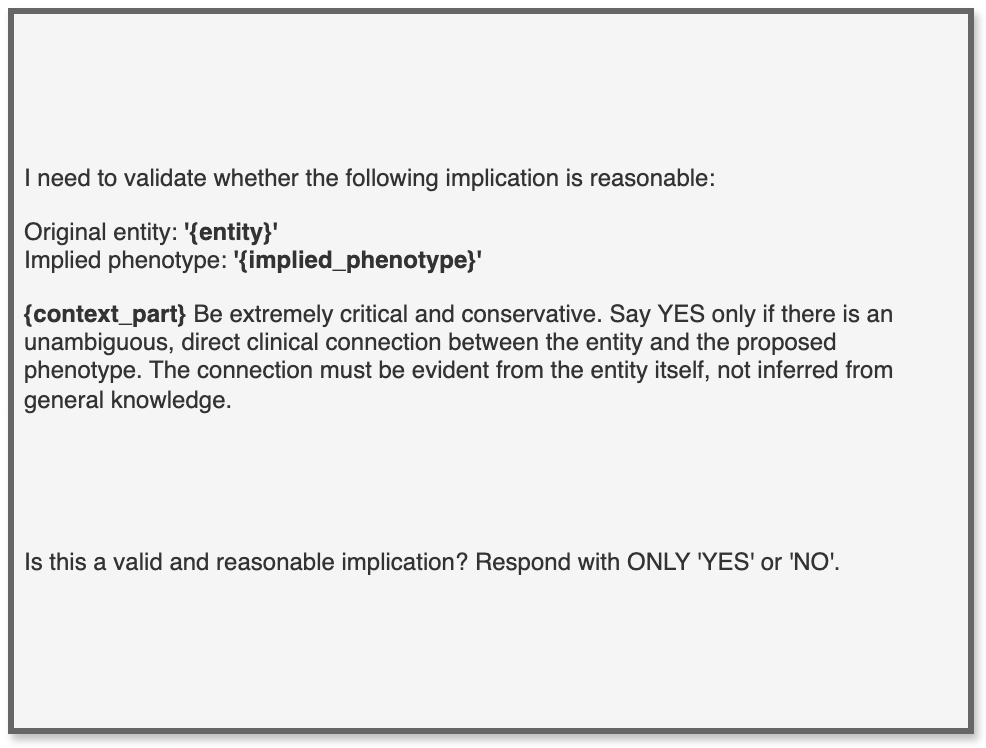
\includegraphics[width=0.8\textwidth]{figs/prompts/hpo/PhenotypeImplicationReasonable.drawio.png}
    \caption{\textbf{Phenotype Implication Reasoning Check.} The LLM is then asked to double check its implication to make sure it makes sense.}
    \label{fig:PhenotypeImplicationReasonableCheck}
\end{figure}

\begin{figure}[h!]
    \centering
    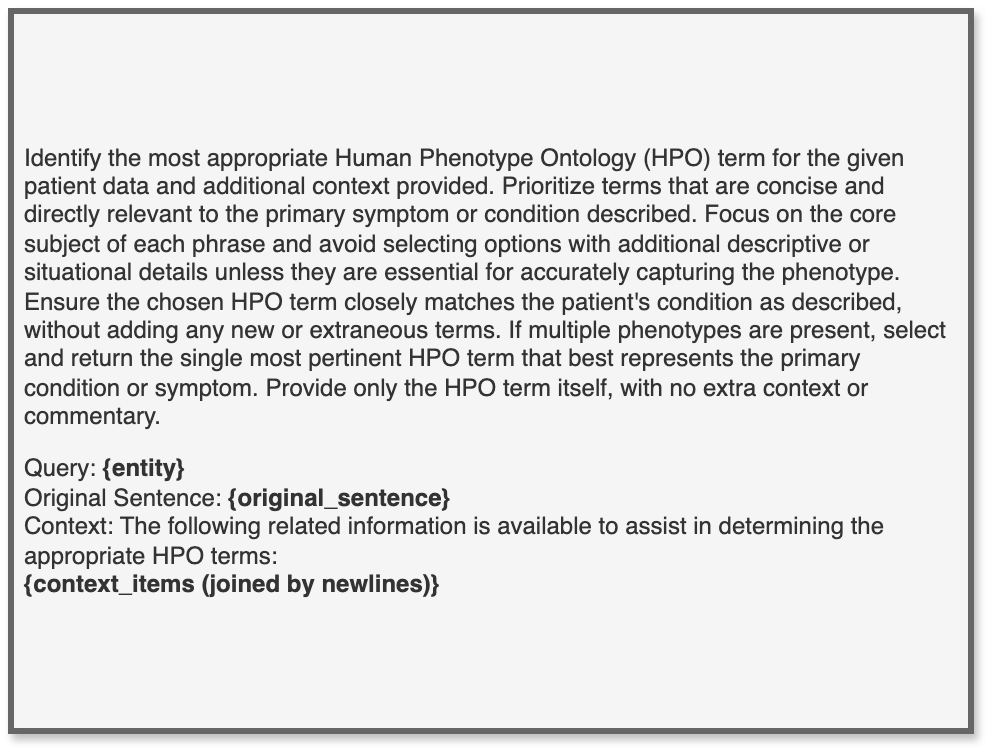
\includegraphics[width=0.8\textwidth]{figs/prompts/hpo/PhenotypeMatching.drawio.png}
    \caption{\textbf{Phenotype Matching.} Finally, the LLM is asked to match the an entity or implied entity to a matching phenotype.}
    \label{fig:PhenotypeMatching}
\end{figure}

\clearpage
\subsection{Rare Disease Verification and Matching Prompts} \label{appendix: rd prompts}

\begin{figure}[h!]
    \centering
    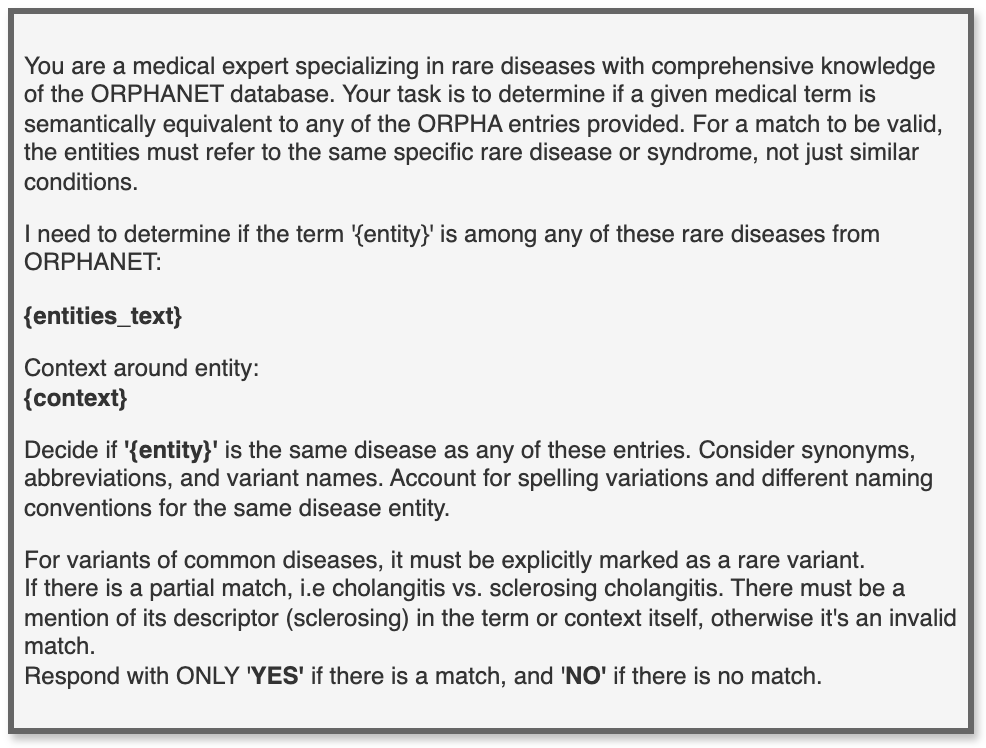
\includegraphics[width=0.8\textwidth]{figs/prompts/rd/RDOntologyCheck.drawio.png}
    \caption{\textbf{Rare Disease Entity Ontology Check.} This prompt checks if the entity is within the Orphanet ontology.}
    \label{fig:RDOntologyCheck}
\end{figure}

\begin{figure}[h!]
    \centering
    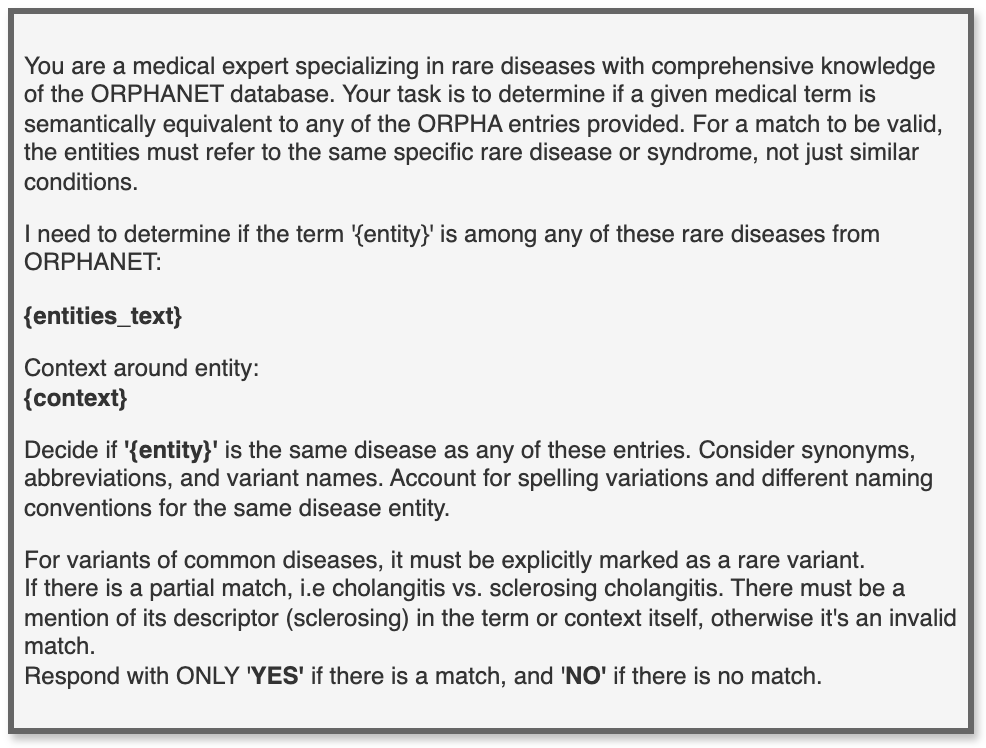
\includegraphics[width=0.8\textwidth]{figs/prompts/rd/RDOntologyCheck.drawio.png}
    \caption{\textbf{Rare Disease Check.} This prompt checks if the entity is actually disease, because not all Orphanet entities are diseases. }
    \label{fig:RDDiseaseCheck}
\end{figure}

\begin{figure}[h!]
    \centering
    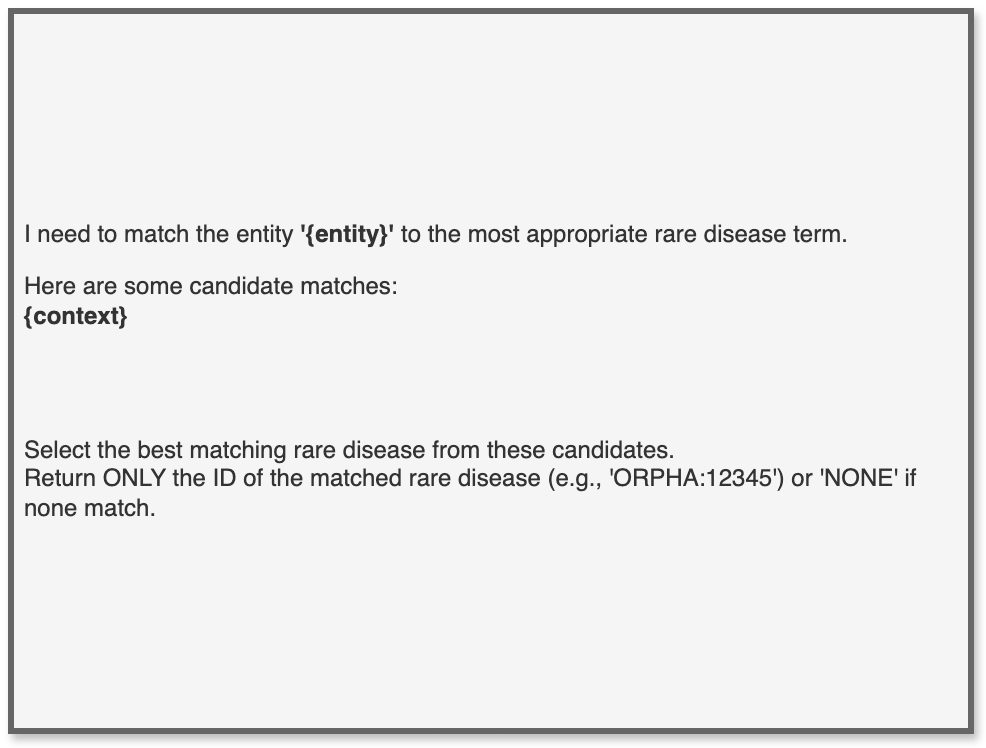
\includegraphics[width=0.8\textwidth]{figs/prompts/rd/RDMatch.drawio.png}
    \caption{\textbf{Rare Disease Matching.} This prompt matches the verified entity to an Orpha code.}
    \label{fig:RDMatch}
\end{figure}


\rev{\subsection{Performance Across Annotation Sets} \label{appendix: rd annotations perf}}
\rev{We disclose what performance metrics look like across the original noisy set of annotations and our different variants of corrected annotations here.}

\begin{table}[h]
\centering
\resizebox{0.8\textwidth}{!}{%
\begin{tabular}{l c c c c}
\hline
\textbf{Baseline} & \textbf{Model} & \textbf{Precision} & \textbf{Recall} & \textbf{F1} \\
\hline
0-shot & Llama 3.3 70B$^q$ & 0.01 & 0.03 & 0.02 \\
Retrieve and String Match & MedEmbed & 0.23 & 0.36 & 0.28 \\
RAG-RD & Mistral 24B$^q$ & 0.17 & 0.45 & 0.24 \\
RDMA & Mistral 24B$^q$ & \textbf{0.67} & \textbf{0.28} & \textbf{0.39} \\
\hline
\multicolumn{5}{c}{\textbf{Human Corrected Labels}} \\
\hline
0-shot & Llama 3.3 70B$^q$ & 0.01 & 0.05 & 0.02 \\
Retrieve and String Match & MedEmbed &  0.25 & 0.43 & 0.32 \\
RAG-RD & Mistral 24B$^q$ & 0.14 & \textbf{0.54} & 0.22 \\
RDMA & Mistral 24B$^q$ & \textbf{0.66} & 0.38 & \textbf{0.48} \\
\hline
\end{tabular}%
}
\caption{\textbf{Rare Disease Extraction Performance Comparison.} We showcase performance on the other 2 sets of rare disease mention labels, the noisy original and the human only corrected labels. We observe that RDMA has significantly higher precision than its baselines, and that it overall outperforms all of its baselines in F1. \textbf{Bold} denotes best performance.}
\label{tab:label_correction}
\end{table}
